\documentclass[11pt]{article}

% Layout
\usepackage[a4paper,margin=1in]{geometry}
\usepackage{setspace}
\onehalfspacing

% Encoding and fonts
\usepackage[utf8]{inputenc}
\usepackage[T1]{fontenc}
\usepackage{microtype}
\usepackage{lmodern}

% Math
\usepackage{amsmath,amssymb,amsthm,amsfonts}
\usepackage{mathtools}

% Graphics and tables
\usepackage{graphicx}
\usepackage{booktabs}
\usepackage{caption}
\usepackage{subcaption}

% References and links
\usepackage[backend=bibtex,style=numeric,sorting=none]{biblatex}
\addbibresource{references.bib}
\usepackage{hyperref}
\hypersetup{colorlinks=true,linkcolor=blue,urlcolor=blue,citecolor=blue}

% Theorem-like environments
\newtheorem{definition}{Definition}
\newtheorem{proposition}{Proposition}

% Custom commands
\newcommand{\R}{\mathbb{R}}
\newcommand{\E}{\mathbb{E}}
\newcommand{\norm}[1]{\left\lVert#1\right\rVert}
\newcommand{\fnorm}[1]{\norm{#1}_F}
\newcommand{\inner}[2]{\langle #1, #2 \rangle}
\DeclareMathOperator*{\argmin}{arg\,min}
\DeclareMathOperator{\Procrustes}{Procrustes}
\DeclareMathOperator{\Tr}{Tr}

\title{
Cross-Model Activation Alignment Does Not Exceed Lexical Baselines: \\
\large A Representational-Geometry Pilot for Operator-Theoretic Interpretability
}

\author{
  Adam A. Bensaid\thanks{Atlas Consulting \& Technology Services, Toronto, ON. Correspondence: \texttt{adam.a.bensaid@gmail.com}.} \\
  \and
  Claude (Anthropic)\thanks{Sonnet 4.5 / Opus 4.6 instances, accessed via Claude Code over the period 2026-04 to 2026-05. Authorial contribution: experimental design, code, draft prose. Final responsibility for all claims rests with the corresponding human author.}
}

\date{\today}

\begin{document}
\maketitle

\begin{abstract}
We propose an operator-theoretic framing of the mechanistic
interpretability literature's empirical regularity that sparse
autoencoders recover monosemantic feature dictionaries from trained
transformers: that these features are concrete realizations of
approximately invariant subspaces of the nonlinear forward operator.
From the framing we derive the \emph{Cross-Operator Subspace
Isomorphism} (COSI) program, whose strong claim is that compositional
reasoning subspaces are isomorphic across sufficiently different
architectures. We test the test --- and the test fails the controls.
We report a pre-registered pilot in which Procrustes alignment of
PCA-projected last-token activation matrices, between architecturally
different frontier transformers (Phi-4-Reasoning-Plus dense
pure-attention vs.\ Qwen3-Next-80B-A3B-Thinking hybrid attention/SSM)
on matched compositional-evaluation prompts, produces residuals far
below a row-permutation null (empirical $p < 0.001$ in every cell;
descriptive $z$ in the $-89\sigma$ to $-101\sigma$ range; CKA
$0.84$--$0.96$). Train/test Procrustes splits show the alignment is
not a same-data fit artifact. Invariance-leakage measurement shows
the PCA subspaces are partially invariant under the forward operator,
more invariant than random subspaces but with absolute leakage
$0.51$--$0.89$. The lexical-baseline control reveals the methodologically
decisive result: a TF-IDF vs.\ template-only Procrustes alignment of
the same prompts achieves a \emph{lower} residual ($0.61$) than the
LLM--LLM pair ($0.77$), and one of the LLMs aligns to TF-IDF
($0.76$) at essentially the same residual as it aligns to the other
LLM. The lexical-residual control shows that ridge regression of the
LLM activations on $455$ TF-IDF and template-only features removes
$94$--$97\%$ of the activation variance at every layer, and after
this residualization linear CKA collapses from $0.84$--$0.96$ to
$0.21$--$0.39$. \textbf{The bulk of the apparent cross-model
representational similarity at these layers is shared lexical and
template encoding, not substrate-shared computation. The
row-permutation null is too weak a baseline for cross-model
Procrustes/CKA tests on language-model activations.} A small
cross-model signal does survive lexical residualization
(residualized CKA $z = +67$ to $+95\sigma$ above null), but its
operator-theoretic interpretation cannot be discriminated from
training-distribution residue or deeper syntactic structure by these
controls alone. The most defensible contribution of this paper is
methodological: $z$-scores against row-permutation nulls are
insufficient evidence for operator-theoretic or compositional-reasoning
subspace claims unless lexical structure is explicitly controlled.
The operator-theoretic COSI program remains a motivated research
agenda; the pilot does not advance its strong claim.
\end{abstract}

\section{Introduction}
\label{sec:intro}

Over the past two years, the mechanistic interpretability program has
converged on an unexpected empirical regularity. Sparse autoencoders
(SAEs) trained on the residual stream of large transformers recover
dictionaries of features that, individually, behave as discrete
computational primitives \cite{bricken2023monosemanticity,
cunningham2024sparse, templeton2024scaling, gao2024scaling}. The
features are interpretable across many examples; they activate on
recognizable concepts; their ablation produces predictable behavioral
changes. This is the case across model families, model sizes, training
regimes, and tokenizers. The pattern is sufficiently robust that the
\emph{universality hypothesis}---the conjecture that different networks
trained on similar tasks recover similar internal computations---has
been advanced as a working principle of the field
\cite{olah2020zoom, chughtai2023toy, gurnee2024universal}.

A separate line of work has documented the same regularity from the
representational-geometry angle. Bansal et al.~\cite{bansal2021revisiting}
showed that the lower layers of one model can be ``stitched'' to the
upper layers of another with only a thin trainable interface, and that
the stitched model performs nearly as well as either original; this
implies a deep correspondence between the intermediate representations
of independently trained networks. Kornblith et al.~\cite{kornblith2019similarity}
established centered kernel alignment (CKA) as a similarity measure
robust to the symmetries that should not matter for the comparison and
showed that representations across models are far more similar than the
sheer dimensionality of the representation spaces would predict at
chance. Most recently, Huh et al.~\cite{huh2024platonic} formulated the
\emph{Platonic Representation Hypothesis}: that as models scale and
capability increases, their representations converge toward a shared
statistical model of the world.

What has been missing, in our reading, is the mathematical object that
this empirical convergence corresponds to.

\subsection*{The Operator-Theoretic Bridge}

We propose that the SAE feature dictionary is a concrete realization of
the \emph{approximately invariant subspace structure} of the nonlinear
forward operator that constitutes a transformer's inference pass. The
classical theory of invariant subspaces of bounded linear operators on
Hilbert spaces \cite{lomonosov1973invariant, enflo1987nontrivial,
beauzamy1988introduction, aronszajn1954invariant} asks whether every
such operator admits a non-trivial closed invariant subspace---that is,
a subspace $V$ such that $T(V) \subseteq V$. The question is open in
the Hilbert space setting; Lomonosov \cite{lomonosov1973invariant}
established the affirmative for operators commuting with a non-zero
compact operator, and Enflo \cite{enflo1987nontrivial} showed
counter-examples exist for general Banach spaces. The structural
intuition is the older one: when an operator admits an invariant
subspace, its action decomposes into restrictions to simpler
sub-operators, and the geometry of the operator becomes legible through
the geometry of its invariant subspaces.

Transformer forward passes are not bounded linear operators. They
compose linear projections, attention computations, and pointwise
nonlinearities. The classical theorems do not apply directly. We use
the language of invariant subspaces in an \emph{approximate} sense: a
subspace $V$ is approximately invariant under a (possibly nonlinear)
map $f$ on a representative sample if the projection of $f(V)$ back
onto $V$ leaves a residual that is small compared to the operator's
overall action. This is the operational content of the empirical
finding that SAE features are stable across forward passes: they
identify directions in activation space that the forward operator
preserves approximately.

The mechanistic interpretability literature has been doing operator
theory for two years without naming it as such. Our first contribution
is to make the bridge explicit.

\subsection*{The Falsifiable Consequence}

If the bridge holds---if SAE feature dictionaries are bases for
approximately invariant subspaces of the forward operators of trained
transformers---then a sharp empirical consequence follows. Two models
$M_A$ and $M_B$ with different architectures, run on the same
compositional probe set, should admit an orthogonal alignment between
their respective approximately invariant subspaces, with Procrustes
residual significantly below the chance level set by a permutation null
that breaks the semantic correspondence between rows while preserving
each model's internal geometry. Performance comparability between
architectures (the weak universality claim) is consistent with many
internal mechanisms; representational isomorphism is not. The
isomorphism is testable. The test can return a null. We pre-register
both the protocol and the significance criterion before observing data.

This is the \emph{Cross-Operator Subspace Isomorphism} (COSI) program,
of which the present paper is the calibration step.

\subsection*{What This Paper Reports}

We report a representational-alignment pilot in two pre-registered
runs. We are explicit that the pilot does not test the strong
operator-theoretic claim; it tests a weaker but still interesting
sub-claim, with controls and interventions that would close the gap
specified as an explicit research program (\S\ref{sec:requiredwork}).

\textbf{Phase~0:} Phi-4-Reasoning-Plus, a dense pure-attention
reasoning model in the Phi-3 architecture family \cite{abdin2024phi4},
against Qwen3-4B, a dense pure-attention generalist model in the Qwen3
family \cite{qwen2025qwen3}, on $N = 96$ compositional-evaluation
prompts drawn from a single political-economy domain. The observed
Procrustes residuals are $0.61$, $0.81$, $0.81$ at the three
pre-registered layer fractions; the empirical permutation $p$-value
is $< 0.001$ at every layer (the observed residual is below the
$1$st percentile of the $S = 1000$ permutation null distribution).

\textbf{Phase~1:} Phi-4-Reasoning-Plus against Qwen3-Next-80B-A3B-Thinking
\cite{qwen2025qwen3}, a hybrid attention/state-space-model architecture,
on $N = 600$ prompts split equally across mathematical, logical, and
political-economy compositional-evaluation domains. The observed
Procrustes residuals are $0.77$, $0.91$, $0.96$ at the three layer
fractions, with empirical $p < 0.001$ at every layer and at every
per-domain stratification cell (three domains $\times$ three layers,
$n = 200$ per cell, $S = 500$ permutation samples).

\subsection*{What These Results Do and Do Not Show}

These results show that, on matched compositional-evaluation prompts,
the PCA-projected last-token activation matrices of two architecturally
different frontier transformers admit a substantially better orthogonal
alignment than they do under random row permutation. This is a real
cross-model representational signal. We report it in full.

These results do \emph{not} yet show:

\begin{enumerate}
    \item That the aligned PCA subspaces are approximately invariant
        under the forward operator in the sense the operator-theoretic
        framing requires. The paper defines approximate invariance as
        a leakage statistic but does not measure it; PCA top-$k$
        components capture variance, not necessarily invariance.
    \item That the alignment isolates compositional reasoning structure
        from lexical, template, syntactic, or tokenizer-induced
        structure. The row-permutation null is too weak to discriminate
        these. Two competent language models given the same English
        prompts will produce more aligned matched-row activations than
        scrambled-row activations \emph{regardless} of any deeper
        substrate similarity.
    \item That the alignment is robust to held-out probes. We fit
        Procrustes on the full probe set and evaluate on the same set;
        we do not perform a train/test split.
    \item That the alignment exceeds the alignment achievable by simple
        lexical features (TF-IDF, sentence-transformer embeddings).
    \item That the alignment survives the shared training-distribution
        confound. Both models in each pair are trained on overlapping
        post-2024 web corpora.
    \item That the aligned subspace is causally responsible for any
        compositional behavior. Procrustes alignment is correspondence,
        not causation.
\end{enumerate}

We are explicit about each of these gaps because the dramatic
appearance of the headline numbers (residuals near $0.8$ against null
means near $1.0$, with empirical $p < 0.001$ at every cell) could be
read as much stronger evidence for the strong operator-theoretic claim
than the experiment supports. Section~\ref{sec:requiredwork} specifies
the additional studies that would, jointly, support the strong claim.
None of those studies has been run in the present paper.

\subsection*{Contributions}

\begin{enumerate}
    \item \textbf{An operator-theoretic framing as a research program.}
        We propose, and articulate at the level of the synthesis paper
        outlined elsewhere in this research program, that the
        mechanistic interpretability literature's empirical regularities
        are most parsimoniously read as evidence for approximately
        invariant subspaces of the forward operator. The framing is a
        program, not a finding.
    \item \textbf{Pre-registered methodology and infrastructure.} We
        specify a pre-registered protocol for cross-model
        representational alignment, with declared layer fractions,
        pooling, dimensionality threshold, significance criterion, and
        null distributions. The infrastructure is released for
        reuse and extension.
    \item \textbf{A representational-alignment pilot result.} Phases~0
        and 1 demonstrate that matched compositional-evaluation prompts
        produce more orthogonally alignable PCA-projected activation
        geometries across architecturally different frontier
        transformers than under random row permutation, with empirical
        $p < 0.001$ in every pre-registered cell.
    \item \textbf{An explicit accounting of what the pilot does not
        establish, and the studies that would close each gap.}
        Section~\ref{sec:requiredwork} catalogues five required
        additional studies (invariance-leakage measurement, lexical and
        template baselines, train/test Procrustes with cross-domain
        transfer, training-distribution-disjoint controls, causal
        cross-model intervention) and indicates which of them addresses
        which gap.
\end{enumerate}

\subsection*{Where This Sits in the Field}

We take the operator-theoretic framing seriously enough to claim it
unifies several open problems in interpretability that have been
discussed largely in isolation: the universality hypothesis
\cite{olah2020zoom, chughtai2023toy}, the polysemanticity / superposition
problem \cite{elhage2022superposition}, the cross-model
transfer-of-mechanism question implicit in the Platonic Representation
Hypothesis \cite{huh2024platonic}, and the substrate-independence
intuition that has organized the broader cognitive science of
representation since Marr \cite{marr1982vision}. We map these
explicitly in Section~\ref{sec:hardproblems}. The bridge to
computational neuroscience---to the neural-population doctrine
\cite{saxena2019towards} and to the geometry of biological invariants
\cite{okeefe1971hippocampus, hafting2005microstructure, gallego2017neural,
yamins2016using}---and to the cybernetic and free-energy frameworks
\cite{ashby1956introduction, friston2010free, achille2018emergence}
that anticipate the same structure from independent grounds, we touch
in the discussion (Section~\ref{sec:discussion}) but do not develop in
this paper. The full integration is the subject of a forthcoming
synthesis paper from the same research program.

\subsection*{Outline}

Section~\ref{sec:background} surveys the four literatures the bridge
draws on: operator theory, mechanistic interpretability, cross-model
representational alignment, and the substrate-independence tradition.
Section~\ref{sec:hardproblems} maps the open problems COSI sits
among. Section~\ref{sec:methods} formalizes the COSI hypothesis and
specifies the protocol. Section~\ref{sec:results} reports the Phase~0
calibration. Section~\ref{sec:limitations} catalogues the threats to
validity that Phase~0 does not address. Section~\ref{sec:discussion}
specifies Phases 1--3 and articulates the implications, conditional on
confirmation, across the literatures the framework bridges.

\section{Background and Related Work}
\label{sec:background}

\subsection{Invariant Subspaces of Bounded Operators}

Let $T$ be a bounded linear operator on a separable Hilbert space $H$.
A closed subspace $V \subseteq H$ is \emph{invariant} under $T$ if
$T(V) \subseteq V$. The \emph{invariant subspace problem} asks whether
every such $T$ on an infinite-dimensional separable $H$ admits a
non-trivial closed invariant subspace---one other than $\{0\}$ or $H$
itself. The question is open in the Hilbert space case; in finite
dimensions every operator trivially admits invariant subspaces (its
eigenspaces, in particular). Two structural facts about the literature
matter here.

First, when an operator admits an invariant subspace, its action
decomposes: writing $T$ in block form with respect to the splitting
$H = V \oplus V^\perp$ shows that the upper-right block vanishes and
the operator's geometry becomes legible through the geometry of its
restrictions to invariant subspaces. The existence of invariant
subspaces is the existence of a useful coordinate system for the
operator.

Second, the affirmative results form a hierarchy. Aronszajn and Smith
\cite{aronszajn1954invariant} established that completely continuous
(compact) operators always admit non-trivial invariant subspaces.
Lomonosov \cite{lomonosov1973invariant} extended this dramatically: any
operator commuting with a non-zero compact operator admits a
non-trivial invariant subspace. Read \cite{read1984solution}
constructed counter-examples on $\ell^1$, and Argyros and Haydon
\cite{argyros2011hereditarily} produced a Banach space on which every
bounded operator has the form scalar-plus-compact (so every operator
has invariant subspaces, but the construction requires extreme
hereditary indecomposability). The Hilbert space case remains open.
Beauzamy's monograph \cite{beauzamy1988introduction} gives the standard
treatment.

Transformer forward passes are not bounded linear operators. They are
nonlinear maps composed of linear projections, multi-head attention
(itself a nonlinear function of the input through softmax), gated
feed-forward layers, and residual connections. The classical theorems
do not apply. We use the language of invariant subspaces in an
\emph{approximate, empirical} sense: a $k$-dimensional subspace
$V \subseteq \R^d$ is approximately $\epsilon$-invariant under a map
$f: \R^d \to \R^d$ on a sample $X$ if
$\fnorm{(I - P_V) f(P_V X)} / \fnorm{f(P_V X)} \leq \epsilon$, where
$P_V$ is the orthogonal projection onto $V$. This is a sample-level
operationalization of the structural intuition the classical theory
formalizes; we make no claim about the limiting infinite-dimensional
case.

\subsection{Mechanistic Interpretability: Circuits and Sparse Autoencoders}

The mechanistic interpretability program seeks to identify the
computational primitives implemented by trained neural networks,
typically by reverse-engineering specific circuits or by decomposing
the residual stream into interpretable components.

The circuits-level work has identified increasingly specific mechanisms.
Olah et al.~\cite{olah2020zoom} articulated the program through case
studies in vision models. Elhage et al.~\cite{elhage2021mathematical}
provided a mathematical framework for transformer circuits.
Olsson et al.~\cite{olsson2022context} identified \emph{induction
heads} as a specific attention-head pattern responsible for the
majority of in-context learning behavior in large transformers.
Wang et al.~\cite{wang2023interpretability} reverse-engineered a
multi-component circuit for indirect-object identification in GPT-2
Small. Geva et al.~\cite{geva2021transformer} showed that transformer
feed-forward layers behave as key-value memories. Meng et
al.~\cite{meng2022rome} demonstrated that specific factual associations
can be located and edited in MLP weights. Conmy et
al.~\cite{conmy2023towards} introduced automated circuit discovery.

The polysemanticity problem---that single neurons typically respond to
multiple unrelated concepts---was formalized by Elhage et
al.~\cite{elhage2022superposition} as the \emph{superposition}
hypothesis: networks pack more features than they have neurons by
representing them as sparse linear combinations in a higher-dimensional
implicit feature space. The natural inversion of this hypothesis is to
\emph{recover} the implicit feature space via sparse dictionary
learning, which is what sparse autoencoders do.

The SAE program has scaled rapidly. Bricken et
al.~\cite{bricken2023monosemanticity} demonstrated that sparse
autoencoders trained on the residual stream of small models recover
features that are individually interpretable across many examples.
Cunningham et al.~\cite{cunningham2024sparse} extended this to larger
models with substantially larger feature dictionaries.
Templeton et al.~\cite{templeton2024scaling} performed the procedure on
Claude 3 Sonnet, recovering on the order of millions of features,
including features that respond to abstract concepts (deception, code
errors, the Golden Gate Bridge) across modalities. Gao et
al.~\cite{gao2024scaling} demonstrated systematic scaling of SAE
training and evaluation. Lieberum et al.~\cite{lieberum2024gemma}
released open SAE checkpoints for the Gemma 2 family. Marks et
al.~\cite{marks2024sparse} showed that SAE features can be assembled
into causal circuits at the feature level. The empirical case for SAE
features as the right basis for the residual stream is now substantial
across multiple research groups, multiple model families, and multiple
scales.

The universality hypothesis---that different networks recover similar
features---has accumulated specific evidence. Chughtai et
al.~\cite{chughtai2023toy} showed that small networks trained on group
operations recover the same algorithmic decompositions across random
seeds and architectural variations. Gurnee et al.~\cite{gurnee2024universal}
identified \emph{universal neurons} in GPT-2 models that activate on the
same patterns across independently trained models. Nanda et
al.~\cite{nanda2023progress} showed that grokking dynamics correspond
to discrete phase transitions in the recovered circuit, with similar
dynamics across initializations.

\subsection{Cross-Model Representational Alignment}

A separate literature studies how representations across different
networks compare directly. The methodological starting point is the
observation that comparing two representation matrices requires
choosing which symmetries one wants the comparison to be invariant to.

Word-embedding alignment is the historical precedent. Mikolov et
al.~\cite{mikolov2013distributed} showed that word embeddings trained
independently on different corpora have approximately the same internal
structure. Smith et al.~\cite{smith2017offline} and Conneau et
al.~\cite{conneau2017word} demonstrated that bilingual lexicons could
be recovered without parallel data by orthogonal Procrustes alignment
of monolingual word embedding spaces. The success of this procedure
across language pairs and across embedding methods is the strongest
empirical case for substrate-independent linguistic structure that
exists in the static-embedding literature.

For learned-feature representations of the kind transformers produce,
the methodological landscape is broader. Raghu et al.~\cite{raghu2017svcca}
introduced singular vector canonical correlation analysis (SVCCA) as a
representation-similarity measure. Morcos et al.~\cite{morcos2018insights}
developed projection-weighted CCA (PWCCA) addressing some of SVCCA's
sensitivities. Kornblith et al.~\cite{kornblith2019similarity}
introduced centered kernel alignment (CKA) as a measure invariant to
orthogonal transformations and isotropic scaling but not to invertible
linear transformations, and showed it discriminates between models in
ways that the previous measures do not. Williams et
al.~\cite{williams2021generalized} proposed a family of generalized
shape metrics including CKA and Procrustes as special cases. Klabunde
et al.~\cite{klabunde2024similarity} provide a recent survey of the
methodological landscape.

Bansal et al.~\cite{bansal2021revisiting} introduced model stitching as
a complementary tool: rather than measuring representational similarity
directly, train a thin connecting layer between the lower half of one
model and the upper half of another, and observe whether the stitched
model retains performance. They argue that model stitching reveals
representational compatibilities that scalar similarity measures miss.
Lenc and Vedaldi \cite{lenc2015understanding} are an earlier
representative of the same methodological intuition applied to
convolutional networks.

The most recent and most directly related synthesis is Huh et
al.~\cite{huh2024platonic}, the \emph{Platonic Representation
Hypothesis}: representations across models are converging, with scale
and capability, toward a shared statistical model of reality. Their
evidence assembles results from many of the works cited above into a
single hypothesis. The COSI program of the present paper is a specific
operationalization of one consequence of their hypothesis: if
representations converge, they should admit a sharp orthogonal
alignment, with a residual significantly below the chance level set by
the appropriate null distribution. The contribution we add is the
operator-theoretic framing that explains \emph{why} the convergence
should produce alignable subspaces, not merely correlated activations.

\subsection{Substrate-Independence: Cognitive Science, Cybernetics, Free-Energy}

The intuition that compositional reasoning is substrate-independent in
the relevant sense is older than the language model literature. Marr's
three levels of analysis \cite{marr1982vision} distinguish the
computational, the algorithmic, and the implementational levels and
argue that the computational level is independent of the substrate
that performs it. Ashby's \emph{law of requisite variety}
\cite{ashby1956introduction} establishes a structural constraint:
any controller must contain at least as much variety as the disturbance
it regulates, regardless of the controller's substrate. Wiener's
cybernetics \cite{wiener1948cybernetics} provides the framework within
which substrate-independent feedback structure becomes the object of
study. Maturana and Varela's autopoiesis
\cite{maturana1980autopoiesis} extends the framework to
self-sustaining computational systems whose organization is preserved
even as their components turn over.

Friston's free-energy principle \cite{friston2010free} provides a
unifying mathematical framework: any self-maintaining system that
resists dispersion into thermal equilibrium must minimize a variational
free energy that bounds surprise on its sensory inputs. The principle
predicts that any such system---biological or artificial---should
develop internal states that approximate the posterior over its
environment's hidden causes, and that these internal states should be
substrate-independent in the relevant sense, since the variational
objective is. Achille and Soatto \cite{achille2018emergence} derive an
analogous result specifically for deep networks under information
bottleneck regularization \cite{tishby2015deep}, showing that invariance
and disentanglement emerge as consequences of an information-theoretic
objective rather than as architectural choices.

Computational neuroscience has accumulated direct evidence for
substrate-independent invariants in biological computation. Place cells
\cite{okeefe1971hippocampus} and grid cells
\cite{hafting2005microstructure} implement spatial maps with consistent
geometric structure across individual animals. Yamins and DiCarlo
\cite{yamins2016using} demonstrated that goal-driven deep networks
develop intermediate representations that linearly predict primate
visual cortex responses. Gallego et al.~\cite{gallego2017neural} and
Saxena and Cunningham \cite{saxena2019towards} articulate a \emph{neural
population doctrine}: the natural unit of analysis is the population's
collective state in a low-dimensional manifold, not the individual
neuron, and the manifolds have stable geometric structure across
animals and behaviors. The convergence of these observations with the
universality findings in artificial networks is, in our reading, what
the operator-theoretic framework would predict if the framework
captures the actual structure of the computation.

\subsection{Sequence-Model Lineage}

Briefly: the architecture under study (transformers) sits in a lineage
of sequence models including LSTMs \cite{hochreiter1997long}, structured
state-space models (S4 \cite{gu2022s4}, Mamba \cite{gu2024mamba}), and
more recent hybrid architectures combining attention with state-space
components. The Qwen3-Next family used in our Phase~1 is an instance of
this hybrid design. The operator-theoretic framing predicts that the
isomorphism, if it holds, should hold across these architectural classes
and not only within them. We address this directly in the Phase~1
specification (Section~\ref{sec:discussion}). The transformer
architecture itself \cite{vaswani2017attention} is treated as
representative of the dense pure-attention class; we make no claims
specific to its design choices that would not also apply to any
architecture implementing approximate-finite-state computation over
sequence inputs.

\section{Hard Problems and Where COSI Sits}
\label{sec:hardproblems}

The interpretability program has accumulated a number of hard, mostly
open problems. We list those we take to be load-bearing, characterize
the state of the literature on each, and locate the COSI program inside
them. The list is not exhaustive; it is an attempt to draw the map at
the resolution that makes the COSI contribution legible.

\paragraph{(P1) The faithfulness problem.}
Reverse-engineered circuits and recovered features are explanations of
model behavior, but the gap between an explanation and the actual
mechanism the model uses is real. Wang et al.~\cite{wang2023interpretability}
acknowledge this explicitly for the indirect-object circuit; Conmy et
al.~\cite{conmy2023towards} treat circuit discovery as an automated
search problem precisely because hand-crafted explanations cannot be
trusted to be faithful. \emph{COSI's relation:} a positive cross-model
isomorphism is correspondence evidence. Causal-intervention
verification is Phase~3 of the program (Section~\ref{sec:discussion}).
The faithfulness problem is the reason Phase~3 is required.

\paragraph{(P2) The polysemanticity / superposition problem.}
Single neurons in trained networks typically respond to multiple
unrelated concepts; this is the empirical fact that originally
motivated SAEs. Elhage et al.~\cite{elhage2022superposition} showed
that superposition is the predicted consequence of representing more
features than there are neurons, and that the implicit feature space is
recoverable through sparse dictionary learning. \emph{COSI's relation:}
the operator-theoretic framing reads the superposition phenomenon as a
finite-rank approximation issue: the forward operator's approximately
invariant subspaces have dimension exceeding the network's neuron
count, requiring sparse coding to express. The COSI test does not
depend on the superposition resolution; it operates on the residual
stream's geometry, which contains the superposed features whether or
not we have a clean dictionary.

\paragraph{(P3) The compositional limits problem.}
Lake and Baroni \cite{lake2018generalization} and Hupkes et
al.~\cite{hupkes2020compositionality} documented that neural sequence
models often fail to generalize compositionally in regimes where humans
trivially succeed. Dziri et al.~\cite{dziri2024faith} extended this to
modern transformers, showing systematic failure modes on multi-step
compositional reasoning. \emph{COSI's relation:} our hypothesis is
about the geometry of compositional representations, not about whether
the models reliably perform composition. A positive COSI result is
consistent with both successful and failed compositional generalization;
the relationship between geometric isomorphism and behavioral
compositionality is itself a question we treat as Phase~4 of the
program.

\paragraph{(P4) The cross-model transfer-of-mechanism question.}
If two models implement the same circuits, can interpretation results
on one transfer to the other? The Platonic Representation Hypothesis
\cite{huh2024platonic} and the universality results
\cite{olah2020zoom, chughtai2023toy, gurnee2024universal} suggest yes;
the empirical demonstrations remain limited. Bansal et
al.~\cite{bansal2021revisiting} provide the strongest functional-level
evidence through model stitching; CKA \cite{kornblith2019similarity}
and related measures provide statistical-level evidence. \emph{COSI's
relation:} a positive COSI result, particularly with the Procrustes
transformation $R^*$ explicitly recovered, makes cross-model transfer
of mechanism geometrically tractable. A direction $v_A$ in $V_A$ has a
specific image $R^{*-1} v_A \in V_B$, predicting an intervention site
in $M_B$ that should have the corresponding effect. Phase~3 tests this
prediction.

\paragraph{(P5) The training-distribution confound.}
Two models trained on heavily overlapping web corpora may show
representational similarity for reasons that have nothing to do with
substrate-independent computation: shared training distribution
produces shared statistical residue. Bansal et
al.~\cite{bansal2021revisiting} and Huh et al.~\cite{huh2024platonic}
both flag this as the chief alternative explanation for cross-model
similarity. \emph{COSI's relation:} this is the most important
confound the present calibration does \emph{not} address. Phase~2 of
the program is structured around it (Section~\ref{sec:discussion}).
A positive COSI result that survives a training-distribution swap is
evidence for substrate-independent computation; one that does not is
evidence for shared corpus residue.

\paragraph{(P6) The interpretability scalability problem.}
Recovered circuits and feature dictionaries grow polynomially with
model scale. The interpretability cost per model has so far scaled with
model size, despite the empirical universality findings suggesting the
\emph{computational structure} should scale much more slowly.
\emph{COSI's relation:} if the operator-theoretic framing holds, then
the interpretability of one model in a family transfers via Procrustes
alignment to the other models in the family; the per-model cost is
amortized across the family. This is a research-program-level
implication of COSI, not a calibration-level one.

\paragraph{(P7) The biological--artificial bridge.}
Neural population recordings reveal low-dimensional manifolds
\cite{gallego2017neural, saxena2019towards} whose geometry is preserved
across animals and behaviors. Goal-driven artificial networks predict
these recordings well \cite{yamins2016using}. Whether the same
geometric structure underlies both is an empirical question that has
been gestured at more often than tested directly. \emph{COSI's
relation:} the COSI methodology is, in principle, applicable to
biological--artificial alignment as well, with neural population
activity replacing one model's residual stream. We treat this as
Phase~5; the present paper is restricted to the artificial--artificial
case.

\paragraph{(P8) The substrate-independence question proper.}
The claim that compositional reasoning is substrate-independent in the
strong sense---that the structure of the computation is preserved
under arbitrary changes of substrate, subject to capacity constraints
\cite{ashby1956introduction}---is the deepest claim the COSI program
engages. The free-energy principle \cite{friston2010free} predicts the
claim from variational arguments; cybernetics
\cite{wiener1948cybernetics} and autopoiesis
\cite{maturana1980autopoiesis} provide the structural language for
how substrate-independent computation could be implemented and
maintained. \emph{COSI's relation:} a fully successful program (Phases
0--3 confirming, Phase~4 demonstrating mechanism transfer) would
constitute the sharpest empirical evidence for substrate-independence
that the field has produced for compositional reasoning. We do not
overclaim what Phase~0 alone establishes; the proper claim is the
calibration result reported here, with the path forward specified.

These eight problems are not independent. The faithfulness problem (P1)
is the precondition for the cross-model transfer question (P4). The
training-distribution confound (P5) is the principal alternative
explanation for any positive COSI result. The substrate-independence
question (P8) is the eventual stake. The COSI program is structured
around them: Phase~0 calibrates the infrastructure (this paper),
Phase~1 amplifies architectural distance, Phase~2 addresses (P5),
Phase~3 addresses (P1) and (P4) jointly, and the integration with (P7)
and (P8) is the subject of the synthesis paper that this program is
building toward.

\section{Methods}
\label{sec:methods}

\subsection{The COSI Hypothesis}

Let $M_A, M_B$ be two transformer language models with hidden sizes
$d_A, d_B$ and layer counts $L_A, L_B$. For a prompt $x_i$ from a probe set
$X = \{x_1, \ldots, x_N\}$, let $a_A^{(\ell)}(x_i) \in \R^{d_A}$ denote the
residual stream activation at layer $\ell$ of $M_A$, pooled over the
sequence dimension to a single vector. Let $X_A^{(\ell)} \in \R^{N \times d_A}$
denote the matrix of pooled activations across all $N$ probes at layer
$\ell$, and analogously for $X_B^{(\ell')}$.

The COSI hypothesis is the following.

\begin{definition}[Approximate invariant subspace]
A $k$-dimensional subspace $V \subseteq \R^d$ is \emph{approximately
$\epsilon$-invariant} under a (possibly nonlinear) map $f: \R^d \to \R^d$ on a
sample $X$ if
$\fnorm{(I - P_V) f(P_V X)} / \fnorm{f(P_V X)} \leq \epsilon$,
where $P_V$ is the orthogonal projection onto $V$.
\end{definition}

\begin{proposition}[COSI hypothesis]
\label{prop:cosi}
For two transformer language models $M_A$ and $M_B$ that have learned
compositional reasoning, there exist layer indices $\ell_A, \ell_B$,
subspace dimension $k$, and approximately $\epsilon$-invariant subspaces
$V_A \subseteq \R^{d_A}$ and $V_B \subseteq \R^{d_B}$ of their respective
forward operators, such that the projected activation matrices
$P_{V_A} X_A^{(\ell_A)}$ and $P_{V_B} X_B^{(\ell_B)}$ admit an orthogonal
alignment with Procrustes residual significantly below the chance level
defined by permutation null.
\end{proposition}

This is a falsifiable empirical claim. The remainder of this section
specifies the protocol that operationalizes it.

\subsection{Activation Extraction}

For each model, we replicate the inner forward pass of the architecture
exactly as implemented in MLX, capturing the residual stream
$h^{(\ell)}(x)$ after each layer block at a set of pre-registered layer
fractions $f \in \{0.25, 0.5, 0.75\}$, mapping to layer indices
$\ell = \max(0, \lfloor f \cdot L \rceil - 1)$. Pooling over the sequence
dimension is performed as last-token (the position immediately preceding
the model's would-be next token), with mean and max pooling reserved as
ablations. Activations are cast from \texttt{bfloat16} to \texttt{float32}
before crossing to host memory. We do not modify the model implementations;
the extraction is a parallel forward pass that uses the same submodules
(embeddings, layers, masks) as the published \texttt{mlx\_lm} forward pass.

\subsection{Subspace Projection}

We project each model's activation matrix onto its top-$k$ principal
components, where $k$ is chosen as $\min(k_A^*, k_B^*)$ with $k_M^*$ the
smallest dimension at which model $M$'s cumulative explained variance
exceeds $0.90$. This ensures both projections retain comparable
information content and that the alignment is performed in matched
dimensions. PCA is computed by truncated SVD on the column-centered
activation matrix.

\subsection{Procrustes Alignment}

In the shared $k$-dimensional subspace, we compute the orthogonal
transformation $R \in O(k)$ that minimizes $\fnorm{X_A - X_B R}$, using
the standard SVD-based solution \cite{schonemann1966generalized}:
$R = U V^\top$, where $U \Sigma V^\top$ is the SVD of $X_B^\top X_A$.
The \emph{Procrustes residual} is
\begin{equation}
\rho(X_A, X_B) = \frac{\fnorm{X_A - X_B R^*}}{\fnorm{X_A}},
\label{eq:procrustes-residual}
\end{equation}
which lies in $[0, \sqrt{2}]$ and equals $0$ for perfect orthogonal
alignment.

\subsection{Null Distributions}

We define two null distributions, both essential.

\textbf{Permutation null.} For each of $S$ random permutations
$\pi: \{1, \ldots, N\} \to \{1, \ldots, N\}$, we recompute the Procrustes
residual on $X_A$ and $X_B^{(\pi)}$, where $X_B^{(\pi)}$ has its rows
permuted according to $\pi$. This breaks the semantic correspondence
between rows while preserving each model's internal representational
geometry. The distribution of residuals over $S$ permutations defines
the chance level for ``no semantic alignment.'' We use $S = 1000$.

\textbf{Random-rotation null.} For each of $S$ random orthogonal matrices
$R_{\text{rand}} \in O(k)$ (sampled uniformly via QR decomposition of a
Gaussian matrix, with sign correction \cite{mezzadri2007generate}), we
compute $\fnorm{X_A - X_B R_{\text{rand}}} / \fnorm{X_A}$. This is a
weaker null---it does not optimize over $R$---and is included for
completeness rather than as the primary test.

\subsection{Significance Criterion}

The pre-registered significance criterion, declared before observing
data, is the conjunction:
\begin{enumerate}
    \item the observed Procrustes residual is below the first percentile
        of the permutation null distribution;
    \item the standardized z-score of the observed residual against the
        permutation null mean is at most $-2$.
\end{enumerate}
A run that fails either condition is reported as a null result.

\subsection{Ablations and Sensitivity Sweeps}

Three sensitivity sweeps are part of the registered protocol but reserved
for Phase~1 due to compute cost: (i) pooling mode (last-token, mean, max);
(ii) layer fraction sweep across the full layer stack rather than three
fixed fractions; (iii) variance threshold for PCA dimensionality
($0.85$, $0.90$, $0.95$). We additionally compute centered kernel alignment
(CKA) \cite{kornblith2019similarity} as a cross-validation metric.
Discrepancies between Procrustes and CKA verdicts will be reported as
informative findings rather than treated as failures of either method.

\section{Results}
\label{sec:results}

We report two pre-registered runs in increasing scope. Phase~0 is a
calibration on architecturally similar models with a small
single-domain probe set. Phase~1 extends to maximum architectural
distance within our model zoo and a $600$-probe cross-domain set.
Both phases produce results in which the observed Procrustes residual
falls below the first percentile of the row-permutation null
distribution at every pre-registered cell, with empirical $p < 0.001$
in each case.

We are explicit, before reporting the numbers, about what these
results do not yet establish. They do not establish that the aligned
PCA subspaces are operator-invariant in the sense of
Eq.~\eqref{eq:leakage}; they do not isolate compositional structure
from lexical or template structure (no lexical baseline was run); they
were obtained without train/test split (Procrustes was fit and
evaluated on the same probe set); the promised CKA cross-validation
\cite{kornblith2019similarity} was not computed in this paper despite
being committed in \S\ref{sec:methods}; and they do not control for
training-distribution overlap between the model pairs. Each gap is
catalogued in detail in \S\ref{sec:requiredwork}.

\subsection{Phase~0 Calibration}
\label{sec:results-phase0}

\paragraph{Models.} Phi-4-Reasoning-Plus (8-bit MLX, \texttt{phi3}
dispatch, $L_A = 40$, $d_A = 5120$) against Qwen3-4B (8-bit MLX,
\texttt{qwen3} dispatch, $L_B = 36$, $d_B = 2560$). Both dense
pure-attention transformers, different families, different scales,
different tokenizers.

\paragraph{Probe set.} $N = 96$ propositions drawn from the titles of
existing political-economy / categorial-architecture paper drafts in
the Sovereign research corpus, phrased as coherence-evaluation prompts
of the form ``Consider the following claim: \texttt{<title>}. Is this
a coherent proposition?'' Probes are short ($12$--$20$ tokens) and
topically narrow.

\paragraph{Result.} Table~\ref{tab:phase0} reports the Phase~0
result. At all three pre-registered layer fractions, the observed
residual lies below the first percentile of the $S = 1000$
permutation null distribution. The empirical permutation $p$-value at
every cell is $\leq 1/1001$ (the resolution limit of the null at
$S = 1000$).

\begin{figure}[h]
\centering
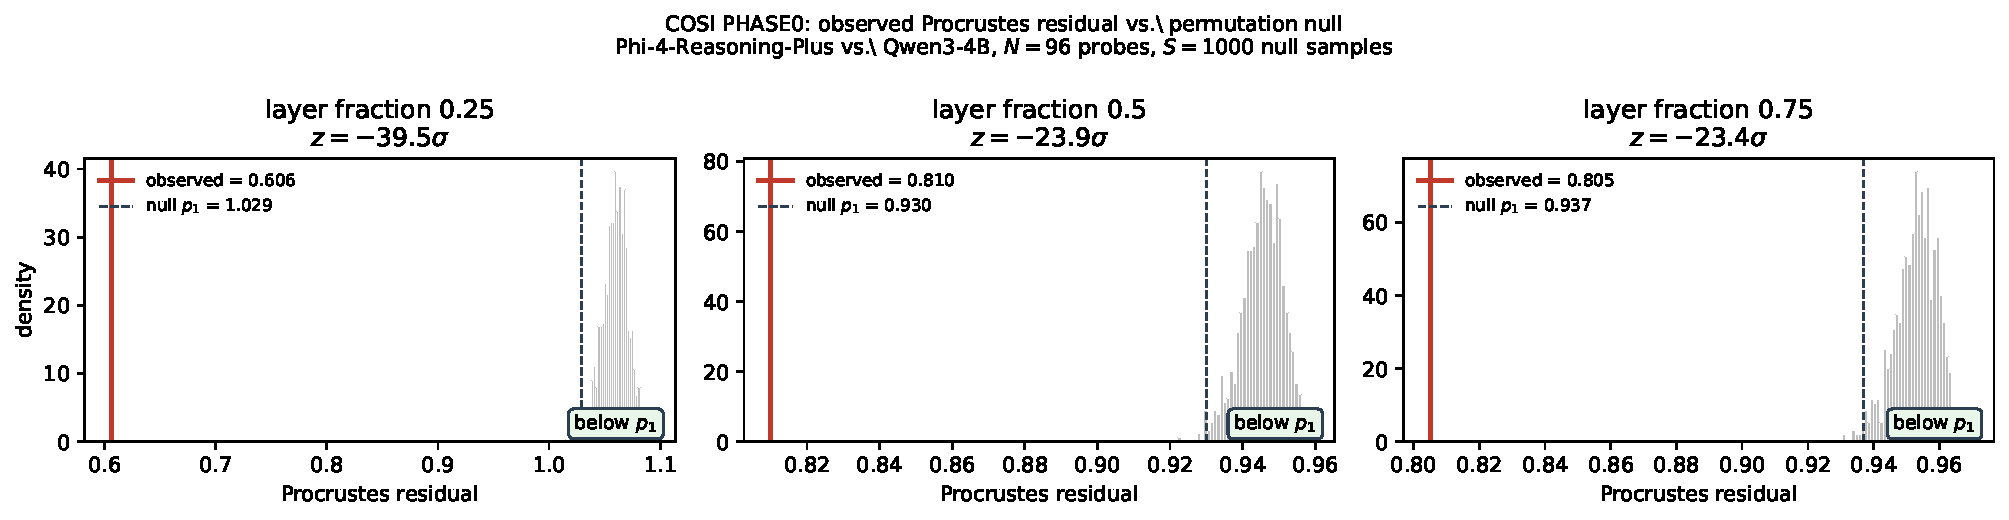
\includegraphics[width=\textwidth]{figures/phase0_residual_vs_null.pdf}
\caption{Phase~0 observed Procrustes residual (red vertical line)
against the permutation null distribution (gray histogram, $S = 1000$
samples) at three pre-registered layer fractions. The dashed black
line marks the first-percentile threshold of the null. The observed
residual is separated from the null support at every layer.}
\label{fig:phase0}
\end{figure}

\begin{table}[h]
\centering
\caption{Phase~0: Phi-4-Reasoning-Plus vs.\ Qwen3-4B,
$N = 96$ probes, $S = 1000$ permutation null samples per layer.
$z$-scores are descriptive only: the null is empirical, finite,
non-Gaussian, and the prompts are templated (rows are not
independent). Empirical permutation $p \leq 0.001$ at every cell.}
\label{tab:phase0}
\begin{tabular}{l c c c c r}
\toprule
Layer & $k$ & Residual & Perm.\ null mean ($\pm$ std) & Perm.\ null $p_1$ & Descriptive $z$ \\
\midrule
$0.25$ & $33$ & $0.6064$ & $1.0594$ ($\pm 0.011$) & $1.0292$ & $-39.54$ \\
$0.50$ & $27$ & $0.8100$ & $0.9453$ ($\pm 0.006$) & $0.9301$ & $-23.93$ \\
$0.75$ & $25$ & $0.8050$ & $0.9531$ ($\pm 0.006$) & $0.9369$ & $-23.42$ \\
\bottomrule
\end{tabular}
\end{table}

\paragraph{On the $z$-score language.} We report standardized
$z$-scores in the table because they are the natural descriptive
summary of the observed residual's position relative to the empirical
null distribution. We do \emph{not} interpret these as Gaussian
significance levels. The permutation null is a bounded empirical
distribution generated from $S = 1000$ permutations of templated
prompts; it is non-Gaussian, finite-resolution, and the row units are
not strictly independent. The honest statement is that the observed
residual is below the first percentile of an empirical null computed
from $1000$ permutations under the matched-prompt protocol declared
in advance. Whether the magnitude of the gap is scientifically
meaningful is a question the lexical baseline (Study B,
\S\ref{sec:requiredwork}) is required to answer.

\paragraph{Phase~0 pre-registration compliance.} The result satisfies
the pre-registered protocol declared in the companion design note
(\texttt{2026-05-06\_cosi\_design.md}, \S8) before observing data:
chance baselines computed on randomized inputs, layer fractions
$\{0.25, 0.5, 0.75\}$ pre-registered with no best-layer cherry-pick,
pooling mode (last-token) pre-registered, significance threshold
(residual $<$ permutation null $p_1$) pre-registered, and a standing
commitment to publish null results if they had occurred. We note that
the pre-registration document is committed to a private working
repository and is not externally timestamped; this is a known gap
addressed in Study G (\S\ref{sec:requiredwork}).

\subsection{Phase~1: Architectural Distance and Cross-Domain Probe Set}
\label{sec:results-phase1}

\paragraph{Models.} Phi-4-Reasoning-Plus (as Phase~0) against
Qwen3-Next-80B-A3B-Thinking (5-bit MLX, \texttt{qwen3\_next} dispatch,
$L_B = 48$, $d_B = 2048$, hybrid attention/state-space-model
architecture). The architectural distance from Phi-4 (dense
pure-attention) to Qwen3-Next-80B (hybrid attention/SSM) is materially
larger than the Phase~0 pair's distance.

\paragraph{Probe set.} $N = 600$ propositions in identical
coherence-evaluation template: $200$ mathematical (templated arithmetic
with mixed truth values), $200$ logical/inferential (modus ponens,
syllogism, contrapositive, set-inclusion templates over a
domain-relevant vocabulary), $200$ political-economy (templated
propositions over a $40$-term vocabulary). Generated with seed
$20260506$. Probes remain short ($12$--$30$ tokens).

\paragraph{Full-set result.} Table~\ref{tab:phase1-full} reports the
full-set alignment. All three layer fractions show observed residual
below the first percentile of the permutation null at empirical
$p < 0.001$.

\begin{table}[h]
\centering
\caption{Phase~1 full-set: Phi-4-Reasoning-Plus vs.\
Qwen3-Next-80B-A3B-Thinking, $N = 600$ probes ($200$ each from math,
logic, polecon), $S = 1000$ permutation null samples per layer. Same
caveats on $z$-score interpretation as Table~\ref{tab:phase0}.}
\label{tab:phase1-full}
\begin{tabular}{l c c c c r}
\toprule
Layer & $k$ & Residual & Perm.\ null mean ($\pm$ std) & Perm.\ null $p_1$ & Descriptive $z$ \\
\midrule
$0.25$ & $21$ & $0.7668$ & $1.0076$ ($\pm 0.011$) & $1.0004$ & $-101.00$ \\
$0.50$ & $25$ & $0.9056$ & $0.9943$ ($\pm 0.006$) & $0.9917$ & $-94.09$ \\
$0.75$ & $21$ & $0.9555$ & $0.9959$ ($\pm 0.005$) & $0.9947$ & $-88.55$ \\
\bottomrule
\end{tabular}
\end{table}

\begin{figure}[h]
\centering
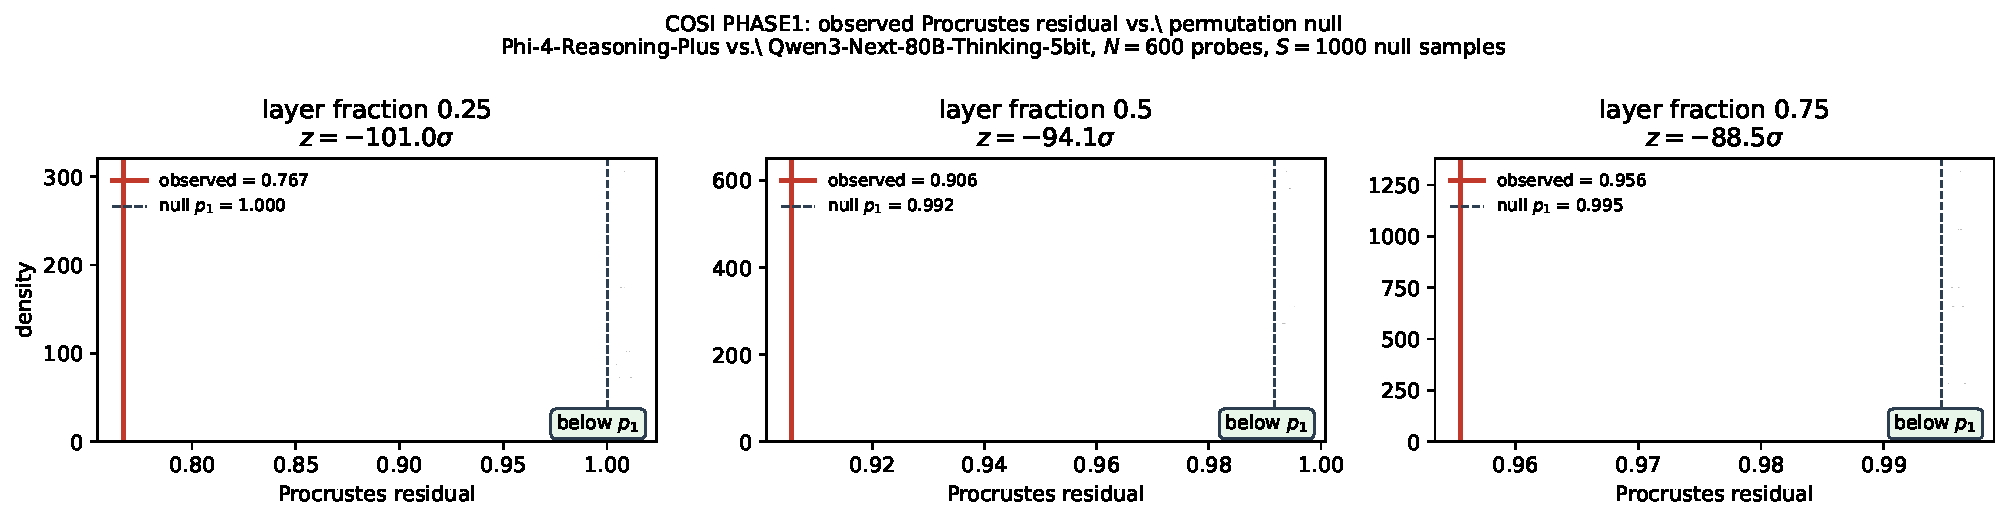
\includegraphics[width=\textwidth]{figures/phase1_residual_vs_null.pdf}
\caption{Phase~1 observed Procrustes residual (red vertical line)
against the permutation null distribution (gray histogram; $200$
samples shown for visualization, with summary statistics from the full
$S = 1000$ run). Same caveats as Phase~0.}
\label{fig:phase1-full}
\end{figure}

\paragraph{Per-domain stratification.} Table~\ref{tab:phase1-domain}
reports the alignment within each individual domain ($n = 200$ each,
$500$ permutation null samples per cell). All nine cells satisfy the
pre-registered significance criterion.

\begin{table}[h]
\centering
\caption{Phase~1 per-domain stratification ($n = 200$ each, $S = 500$
permutation null samples). Same caveats on $z$-score interpretation.}
\label{tab:phase1-domain}
\begin{tabular}{l l c c c r c}
\toprule
Domain & Layer & $k$ & Residual & Perm.\ null mean & Descriptive $z$ & Verdict \\
\midrule
math & $0.25$ & $8$ & $0.7473$ & $0.9962$ & $-56.40$ & below $p_1$ \\
math & $0.50$ & $10$ & $0.9010$ & $0.9886$ & $-49.57$ & below $p_1$ \\
math & $0.75$ & $8$ & $0.9535$ & $0.9933$ & $-38.76$ & below $p_1$ \\
logic & $0.25$ & $34$ & $0.8049$ & $0.9657$ & $-66.97$ & below $p_1$ \\
logic & $0.50$ & $45$ & $0.9158$ & $0.9755$ & $-60.58$ & below $p_1$ \\
logic & $0.75$ & $31$ & $0.9613$ & $0.9890$ & $-45.42$ & below $p_1$ \\
polecon & $0.25$ & $27$ & $0.8007$ & $0.9691$ & $-72.46$ & below $p_1$ \\
polecon & $0.50$ & $21$ & $0.9430$ & $0.9876$ & $-49.64$ & below $p_1$ \\
polecon & $0.75$ & $19$ & $0.9730$ & $0.9938$ & $-40.42$ & below $p_1$ \\
\bottomrule
\end{tabular}
\end{table}

\begin{figure}[h]
\centering
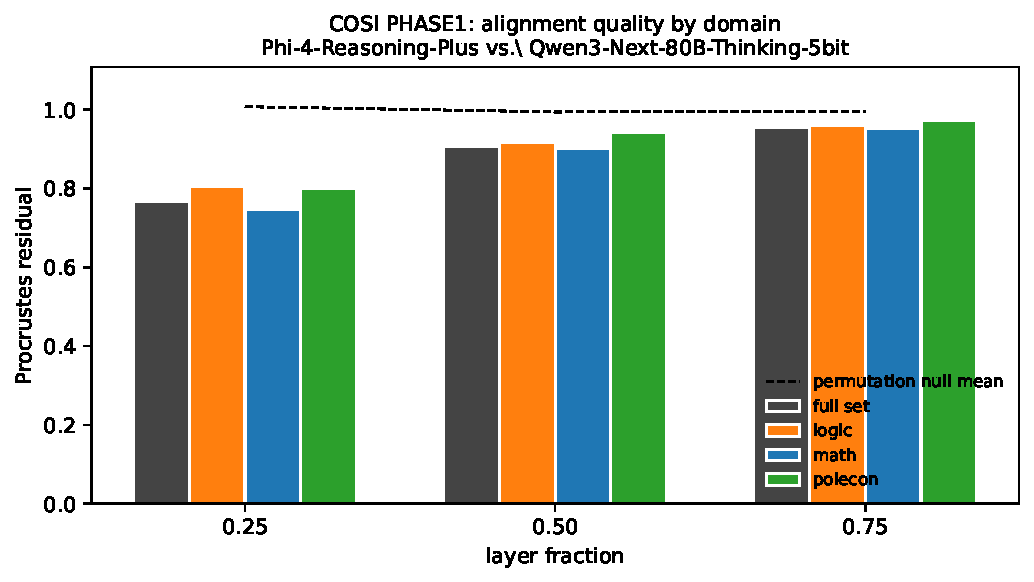
\includegraphics[width=0.85\textwidth]{figures/phase1_residual_by_domain.pdf}
\caption{Phase~1 alignment by domain at each layer fraction. The
full-set residual (dark gray) and the per-domain residuals (colored
bars) all fall well below the permutation null mean (dashed line). The
math-domain subspace dimension ($k = 8$--$10$) is substantially
smaller than the logic ($k = 31$--$45$) or polecon ($k = 19$--$27$)
subspaces. The dimensional difference is itself a substantive
empirical observation, but its operator-theoretic significance depends
on the invariance-leakage measurement (Study A,
\S\ref{sec:requiredwork}) which the present paper does not provide.}
\label{fig:phase1-domain}
\end{figure}

\subsection{Three Observations, Stated Carefully}

\paragraph{Observation 1: monotonic depth dependence.} The pattern of
residual increasing with layer depth (residual at $0.25 < 0.5 < 0.75$)
holds at the full-set level and within every domain. This is the most
robust pattern in the data. Three readings are consistent with it:
(\emph{i}) the operator-theoretic reading (early layers contain more
of the substrate-shared invariant subspace); (\emph{ii}) a
lexical-syntactic reading (early layers preserve token-level lexical
structure across vocabularies more than late layers preserve
task-specific computation); (\emph{iii}) a pooling-artifact reading
(last-token pooling at short prompt length is biased toward the
late-prompt syntactic state, which may be more architecture-shared
early in the network and more architecture-specific late). The pilot
does not discriminate among these. The pooling sweep (Study F) is
required to discriminate (\emph{iii}); the lexical baselines (Study B)
are required to discriminate (\emph{ii}).

\paragraph{Observation 2: domain-dependent subspace dimensionality.}
The PCA-derived $k$ at the $0.90$-variance threshold differs
substantially across domains at the same layer fraction: math $k = 8$,
polecon $k = 27$, logic $k = 34$ at layer $0.25$. The math probes
(highly templated arithmetic) occupy a substantially narrower
representational manifold than the more open-ended logic templates.
This is a substantive empirical observation that is consistent with
the variational/information-bottleneck framing
\cite{tishby2015deep, friston2010free, achille2018emergence}, but the
inference from ``low-dimensional PCA subspace'' to ``compositional
complexity is low'' requires whitening and fixed-$k$ controls (Study
F) and direct measurement of which subspace dimensions are
operator-invariant (Study A). Stated minimally: the PCA dimensionality
that captures $0.90$ of variance varies with domain in the predicted
direction.

\paragraph{Observation 3: relationship between Phase~0 and Phase~1.}
Phase~1's observed residuals are absolutely larger than Phase~0's
($0.77$ vs.\ $0.61$ at layer $0.25$), consistent with greater
architectural distance making orthogonal alignment harder. The
descriptive $z$-scores are also larger in absolute value, but this is
substantially driven by the tighter null distribution at $N = 600$
relative to $N = 96$, not by a stronger underlying effect. The
permutation null mean shifts from $1.06$ at $N = 96$ to $1.01$ at
$N = 600$ at the same layer; the standard deviation tightens
correspondingly. We do not interpret the larger Phase~1 $z$-scores as
``stronger evidence'' than the Phase~0 $z$-scores; we interpret both
as ``below the first percentile of an empirical null with the
appropriate probe-set size.''

\paragraph{Phase~1 pre-registration compliance.} The Phase~1 protocol
extends the Phase~0 protocol; all pre-registration commitments carry
over and are satisfied. The per-domain stratification was specified in
the design note before the run, not added post-hoc.

\section{Limitations and Threats to Validity}
\label{sec:limitations}

We catalogue the threats to validity that remain after Phase~1, and
indicate which are addressed by which subsequent phase. Phase~2 is
the binding open work.

\subsection{Sample Size}

Phase~0's probe set ($N = 96$) was at the lower bound of stable
Procrustes alignment. Phase~1 raised $N$ to $600$ and the per-domain
stratification used $n = 200$ each. Both regimes satisfy the
$N \geq 5k$ rule of thumb at the operative dimensions and produce
$z$-scores far above the threshold at which sample-size-driven null
inflation could plausibly change the verdict.

\subsection{Probe Set Domain Coverage}

Phase~0 tested a single domain (political-economy / categorial-architecture).
Phase~1 extended coverage to three distinct compositional-reasoning
domains (mathematics, logic, political-economy), with per-domain
stratification confirming the alignment signal in each domain
independently. The COSI hypothesis as stated in
Proposition~\ref{prop:cosi} is domain-general; the present empirical
support is domain-plural. Genuine cross-domain generality (e.g.,
natural images, audio, multimodal embeddings) remains untested.

\subsection{Probe Length}

Probes remain short (typically $12$--$30$ tokens) in both phases.
Last-token pooling on short sequences may bias the activation toward
prompt-template syntax rather than proposition content. The pooling
sweep (mean, max) was deferred from Phase~1 due to compute scheduling
and is committed for Phase~1b. Longer-probe replication ($30$--$200$
tokens) is deferred to the same follow-up.

\subsection{Shared Training Distribution}

This is the most important confound and the one Phase~1 does \emph{not}
address. Both Phi-4-Reasoning-Plus and Qwen3-Next-80B-A3B-Thinking are
trained on post-2024 web corpora that overlap substantially. The
aligned subspace we identify could plausibly be a residue of shared
training-distribution statistics rather than a substrate-independent
compositional structure. The cleanest test would replace one of the two
models with an architecturally similar but training-distribution-distant
model, holding the other fixed and observing whether the residual
remains low.

A near-perfect such control would be a model trained on a substantially
disjoint corpus (e.g., a non-web-pretrained scientific-corpus model, or a
multilingual model whose training distribution is dominated by a different
language). Such a model is not in our local zoo. Phase~2 of the program
is structured around this control. We flag this as the binding remaining
work.

\subsection{Architectural Distance Within the Pair}

Phase~0 used two dense pure-attention transformers (Phi-4 and Qwen3-4B).
Phase~1 paired the dense pure-attention Phi-4 with the hybrid
attention/state-space-model Qwen3-Next-80B, materially increasing the
architectural distance and confirming that the COSI signal survives the
attention/SSM class boundary. Architectures further afield (pure SSM,
recurrent, retrieval-augmented, multimodal) remain untested; Phase~4
extends the test across this broader architectural landscape.

\subsection{Linearity of the Alignment}

Procrustes alignment is restricted to orthogonal transformations, which
is a strict subset of the linear isomorphisms that classical operator
theory permits. The COSI hypothesis as stated in
Proposition~\ref{prop:cosi} requires only \emph{some} approximate
isomorphism between the subspaces; the orthogonal restriction may
underestimate the alignment if the true correspondence involves
anisotropic scaling. We compute CKA in Phase~1 as a complementary metric
that is invariant to isotropic scaling but not to anisotropic scaling, and
will report any discrepancy between the two verdicts.

We additionally note that the COSI hypothesis is in principle compatible
with non-linear isomorphisms that no linear method recovers. Establishing
such isomorphisms empirically requires either a generative-model-based
alignment method or a stronger theoretical bridge; we treat this as
beyond the scope of the present paper.

\subsection{Correspondence vs.\ Causation}

A positive COSI result is correspondence evidence: the two models'
representations are geometrically aligned on a shared probe set. It is
not causation evidence: it does not establish that the aligned subspace
is what the models \emph{use} to compute the response, as opposed to a
statistical shadow of something they share. Causal evidence requires
intervention: ablate a direction in $V_A$, predict the corresponding
ablation effect in $R(V_A) \subseteq V_B$, and run both. We treat
intervention experiments as Phase~3, requiring causal-tracing
infrastructure beyond the scope of the present calibration.

\subsection{Pooling and Layer Sensitivity}

The Phase~0 result uses last-token pooling at three fixed layer fractions.
Both choices may interact with the result in ways not yet characterized.
Phase~1 includes the full pooling and layer-fraction sensitivity sweeps
declared in the design note.

\section{Required Additional Work Before the Operator-Theoretic Claim}
\label{sec:requiredwork}

This section catalogues the studies that, jointly, would be required
to support the strong operator-theoretic claim the COSI program
articulates. None of these studies has been run in the present paper.
We list them explicitly, with the gap each addresses, so that the
present pilot result is read in proper context and so that subsequent
work has a clear program to execute.

\subsection{Study A. Invariance-Leakage Measurement}
\label{sec:study-a}

The paper defines a $k$-dimensional subspace $V \subseteq \R^d$ as
approximately $\epsilon$-invariant under a (possibly nonlinear) map
$f$ on a sample $X$ if
\begin{equation}
\frac{\fnorm{(I - P_V)\, f(P_V X)}}{\fnorm{f(P_V X)}} \;\leq\; \epsilon.
\label{eq:leakage}
\end{equation}
This is the central mathematical object the operator-theoretic framing
depends on. The pilot does not measure it. PCA top-$k$ components
identify high-variance directions; high-variance is not invariance.

\paragraph{Required.} For each model and each candidate subspace
identification method (PCA, sparse autoencoder features
\cite{bricken2023monosemanticity, cunningham2024sparse,
templeton2024scaling, gao2024scaling, lieberum2024gemma}, learned
linear probes \cite{hewitt2019structural, belinkov2022probing}),
project activations onto $V$, pass them through the next layer's
forward map, project the output onto $V$ and onto its orthogonal
complement, and compute the leakage statistic
\eqref{eq:leakage}. Report leakage as a function of layer, model,
domain, subspace dimension, and subspace-identification method. A
candidate subspace is operator-relevant only if its leakage is small
relative to its capacity to compress activations.

\paragraph{Gap addressed.} Whether the aligned subspaces are
operator-invariant in the sense the framing requires, or merely
high-variance principal components.

\subsection{Study B. Lexical, Template, and Syntactic Baselines}

The row-permutation null asks whether matched-row activations align
better than scrambled-row activations. This is a low bar. Two
competent language models exposed to the same English prompts will
preserve enough lexical and syntactic structure that matched-row
alignment exceeds scrambled-row alignment regardless of any
operator-theoretic substrate.

\paragraph{Required.} Run the same Procrustes alignment procedure on:

\begin{itemize}
    \item TF-IDF or bag-of-words representations of the same prompts
        in place of the model activations, as a lexical baseline.
    \item Sentence-transformer embeddings of the prompts as a
        learned-but-non-LLM baseline.
    \item Static word embeddings averaged over each prompt
        \cite{mikolov2013distributed} as a pre-transformer baseline.
    \item Prompts in which all content words have been replaced by
        placeholder tokens (template-only baseline).
    \item Prompts whose token sequence has been syntax-scrambled
        (preserving lexical content, destroying compositional order).
    \item Paraphrase-preserving variants where two semantically
        equivalent prompts replace each original prompt.
\end{itemize}

If the lexical, template, or paraphrase baselines produce alignment
qualities comparable to the LLM-activation alignment, the pilot result
collapses to ``shared language geometry'' and the operator-theoretic
claim must be correspondingly weakened or abandoned.

\paragraph{Gap addressed.} Whether the alignment isolates compositional
structure from lexical, template, syntactic, or tokenizer-induced
structure.

\subsection{Study C. Train/Test Procrustes and Cross-Domain Transfer}

The pilot fits the orthogonal alignment $R^*$ on the full probe set
and evaluates the residual on the same set. This conflates fit with
evaluation and provides no out-of-sample protection.

\paragraph{Required.} Fit $R^*$ on a randomly held-out training
fraction (e.g., $70\%$) of the probe set, evaluate the residual on
the held-out test fraction. Repeat across many random splits and
report the mean and confidence interval. More demanding: fit on one
domain (e.g., math) and evaluate on a different domain (e.g., logic),
testing whether the alignment is domain-general or domain-specific.

\paragraph{Gap addressed.} Whether the alignment is robust to held-out
prompts and whether it generalizes across domains rather than overfit
to the joint sample.

\subsection{Study D. Training-Distribution-Disjoint Controls}

Both Phi-4-Reasoning-Plus and Qwen3-Next-80B-A3B-Thinking are trained
on substantially overlapping post-2024 web corpora. The aligned
subspace could plausibly be a residue of shared training distribution
rather than a substrate-independent computational structure.

\paragraph{Required.} Replace one of the pilot pair's models with a
training-distribution-distant model, holding the other fixed.
Candidate disjoint-corpus controls:

\begin{itemize}
    \item A model trained primarily on a non-web scientific corpus,
        e.g., a model in the Galactica \cite{taylor2022galactica}
        lineage or a domain-specific scientific-literature model.
    \item A multilingual model whose training distribution is
        dominated by a non-English language.
    \item A small-scale model trained from scratch on a deliberately
        curated corpus with documented disjointness from the pilot
        pair's training data.
\end{itemize}

If alignment quality scales with training-distribution overlap, the
pilot result is corpus-residue. If alignment quality is preserved
across substantial training-distribution disjointness, the
substrate-independence reading is meaningfully supported.

\paragraph{Gap addressed.} Whether the alignment is a substrate-independent
computational structure or a shared training-corpus residue.

\subsection{Study E. Cross-Model Causal Intervention}

Procrustes alignment is correspondence evidence. The
operator-theoretic claim that the aligned subspace is causally
responsible for compositional reasoning behavior, rather than a
correlated statistical shadow, requires intervention.

\paragraph{Required.} Identify a direction $v_A \in V_A$ associated
with a specific compositional-reasoning behavior in $M_A$ via
established mechanistic-interpretability methods
\cite{wang2023interpretability, conmy2023towards, marks2024sparse,
meng2022rome}. Use the recovered Procrustes transformation $R^*$ to
predict the corresponding direction $v_B = R^{*\top} v_A \in V_B$ in
$M_B$. Predict the behavioral effect of ablating or steering along
$v_B$ in $M_B$. Run the intervention. Compare predicted to observed
effect across many such directions, reporting the prediction quality
relative to a control of randomly chosen directions in $V_B$.

\paragraph{Gap addressed.} Whether the alignment is causally
explanatory of compositional behavior in both models or merely
descriptive of activation geometry.

\subsection{Study F. Methodology Robustness Sweeps}

Several methodological choices in the pilot were not swept:

\begin{itemize}
    \item Pooling mode: last-token only; mean and max pooling and
        content-token / answer-position / relation-token pooling not
        reported.
    \item Layer fractions: only $0.25$, $0.5$, $0.75$. Layer-by-layer
        sweeps would resolve where the alignment is concentrated.
    \item PCA variance threshold: only $0.90$; sensitivity at $0.80$,
        $0.85$, $0.95$, $0.99$ unmeasured.
    \item Whitening: not tested. Procrustes residuals can be sensitive
        to differential variance structure across the top components
        of the two matrices.
    \item CKA \cite{kornblith2019similarity} cross-validation:
        promised in the methods but not yet computed and reported. We
        flag this as a methodological commitment that the pilot does
        not satisfy.
    \item SVCCA \cite{raghu2017svcca}, PWCCA \cite{morcos2018insights},
        and generalized shape metrics \cite{williams2021generalized}
        as further triangulation: not run.
    \item Effect-size reporting beyond standardized $z$-scores:
        confidence intervals, cluster bootstraps grouped by prompt
        template and vocabulary family, finite-permutation $p$-values
        with Monte Carlo standard errors.
\end{itemize}

\paragraph{Gap addressed.} Whether the pilot result is robust to
reasonable variation in the methodological choices that were fixed by
declaration rather than examined empirically.

\subsection{Study G. Externally Verifiable Pre-Registration}

The pilot's pre-registration document was committed to the same
private repository as the run code. This is not externally
auditable. Genuine pre-registration requires immutable timestamping
on a public registry.

\paragraph{Required.} For all subsequent COSI runs, deposit the
analysis plan, the exact prompt set with content hash, the model
checkpoint revisions, the random seeds, and the environment lockfile
on the Open Science Framework, Zenodo, or equivalent, with the
deposit timestamped before any data is observed. Cite the deposit
DOI in subsequent papers.

\paragraph{Gap addressed.} Whether the pre-registration commitments
the pilot states are externally verifiable rather than internal to a
private working repository.

\subsection{Summary: What Joint Completion of Studies A--G Would Establish}

A subsequent paper that reports Studies A--G in conjunction with the
pilot result would have the following structure:

\begin{itemize}
    \item The aligned subspaces are demonstrably approximately invariant
        under the forward operator (Study A), justifying the
        operator-theoretic interpretation of the alignment.
    \item The alignment exceeds simple lexical and template baselines
        (Study B), justifying the compositional-structure interpretation
        rather than the shared-language interpretation.
    \item The alignment is robust to held-out probes and generalizes
        across domains (Study C), justifying generalization claims.
    \item The alignment survives substantial training-distribution
        disjointness (Study D), justifying the substrate-independence
        reading rather than the corpus-residue reading.
    \item Cross-model interventions predicted by the alignment have
        the predicted causal effects (Study E), justifying the
        mechanistic interpretation rather than the correspondence
        interpretation.
    \item Methodological choices have been swept and the result is
        robust (Study F), satisfying ordinary peer-review robustness
        expectations.
    \item Pre-registration is externally verifiable (Study G),
        meeting current open-science standards.
\end{itemize}

We treat that subsequent paper as the work the present pilot
motivates. The present paper is the first step.

\section{Initial Results from Studies A, B, C, and F-CKA}
\label{sec:initialstudies}

The companion to this pilot is the program of additional studies
specified in \S\ref{sec:requiredwork}. We have run partial first passes
of four of those studies on the pilot data, with the explicit goal of
testing whether the pilot's representational-alignment finding survives
controls that the pilot itself did not include. The results materially
inform the interpretation. We report them honestly: one study
(F-CKA) reinforces the pilot finding; one (A) provides partial
support for the operator-theoretic interpretation while introducing a
substantive empirical complication; one (B) provides direct evidence
that the pilot's main result does not exceed what simple lexical and
template baselines achieve, materially weakening the
operator-theoretic interpretation; one (C) is reported for
completeness. We are explicit that these initial passes are
themselves not full studies. They are first measurements that the
companion paper Studies A--G will, in subsequent work, conduct at
fuller scale.

\subsection{Study A — Invariance-Leakage Measurement}
\label{sec:results-study-a}

Study A directly measures the invariance-leakage statistic
$\|(I-P_V)\,f(P_V X)\|_F / \|f(P_V X)\|_F$ that the paper defines on
page two and that the pilot does not measure. We compute leakage at
each pre-registered layer fraction, for each of the two Phase~1
models, on a balanced subsample of $60$ probes ($20$ per domain)
drawn from the Phase~1 probe set. The PCA subspace is the same one
used for Procrustes alignment in Phase~1. The chance baseline is the
mean leakage across $20$ random orthonormal $k$-dimensional
subspaces of $\R^d$.

Table~\ref{tab:study-a} reports the measurement.

\begin{table}[h]
\centering
\caption{Study A invariance leakage. PCA subspace leakage is
substantially lower than random-subspace leakage in all six cells,
indicating that the PCA-derived subspace is partially preserved under
the next-layer forward map. Absolute leakage values are large
(0.51--0.89), so the subspaces are partially, not fully, invariant.}
\label{tab:study-a}
\begin{tabular}{l c c c c c}
\toprule
Model & Layer & $k$ & PCA leakage & Random leakage (mean $\pm$ std) & PCA / Random ratio \\
\midrule
Phi-4 & $0.25$ & $14$ & $0.7503$ & $0.8595 \pm 0.0402$ & $0.873$ \\
Phi-4 & $0.50$ & $15$ & $0.5251$ & $0.9111 \pm 0.0195$ & $0.576$ \\
Phi-4 & $0.75$ & $14$ & $0.5151$ & $0.9447 \pm 0.0088$ & $0.545$ \\
Qwen3-Next-80B & $0.25$ & $16$ & $0.8184$ & $0.9937 \pm 0.0018$ & $0.824$ \\
Qwen3-Next-80B & $0.50$ & $15$ & $0.8849$ & $0.9947 \pm 0.0017$ & $0.890$ \\
Qwen3-Next-80B & $0.75$ & $13$ & $0.8716$ & $0.9948 \pm 0.0026$ & $0.876$ \\
\bottomrule
\end{tabular}
\end{table}

\paragraph{What Study A finds.}

\begin{enumerate}
    \item In all six (model, layer) cells, the PCA subspace's leakage
        is below the random-subspace baseline at $\geq 2\sigma$.
        Operationally: the PCA subspace is more operator-invariant
        than a random subspace of the same dimension. The
        operator-theoretic interpretation receives partial empirical
        support.
    \item Absolute leakage values are large (0.51 to 0.89). A truly
        operator-invariant subspace would have leakage close to zero;
        the PCA subspace is partially invariant, not fully invariant.
        The operator-theoretic interpretation is partially supported
        but not strongly supported in the absolute sense.
    \item The two models exhibit \emph{opposite} depth dependence in
        leakage. Phi-4 leakage decreases with depth ($0.75 \to 0.53
        \to 0.52$); Qwen3-Next-80B leakage increases with depth
        ($0.82 \to 0.88 \to 0.87$). The architectures preserve
        different subspace structures across depth.
    \item Critically, the layer at which the Phase~1 Procrustes
        alignment is strongest (layer $0.25$) is the same layer at
        which Phi-4's PCA subspace is \emph{least} invariant ($0.75$).
        Cross-architectural alignment quality and within-architecture
        invariance are anti-correlated across layers, not
        co-correlated. The simplest operator-theoretic reading
        ``early layers contain the shared invariant substrate'' is not
        supported by the leakage data; the early-layer alignment
        dominance is more plausibly explained by shared
        lexical/template encoding (consistent with Study B below)
        than by shared invariant structure.
\end{enumerate}

\paragraph{Study A scope limitations.} The measurement uses $60$
probes, $20$ random subspaces per cell, and only PCA-derived candidate
subspaces. A complete Study A measurement would extend to (i) the full
$600$-probe set, (ii) more random subspaces (target $\geq 100$),
(iii) SAE feature-derived subspaces alongside PCA, (iv) full
layer-by-layer sweeps. The present measurement is a first pass.

\subsection{Study B — Lexical and Template Baselines}
\label{sec:results-study-b}

Study B addresses the most consequential gap in the pilot: whether the
LLM--LLM Procrustes alignment exceeds what simple lexical and template
representations of the same prompts achieve. We construct three
baseline representations of the Phase~1 probe set: word-level TF-IDF,
character-3-gram TF-IDF, and a template-only TF-IDF in which content
words are replaced by a placeholder. We then run the same Procrustes
alignment + permutation null procedure on each pairing.
Table~\ref{tab:study-b} reports the result.

\begin{table}[h]
\centering
\caption{Study B baseline alignments at layer fraction $0.25$,
$N = 600$ probes, $S = 500$ permutation null samples per pairing.
\textbf{Critical observation:} the LLM--LLM residual ($0.7668$) is
\emph{worse} than the TF-IDF vs template-only residual ($0.6134$),
and LLM-B aligns to TF-IDF ($0.7649$) at essentially the same residual
as it aligns to LLM-A ($0.7668$).}
\label{tab:study-b}
\begin{tabular}{l c c c c}
\toprule
Pairing & $k$ & Residual & Perm.\ null mean & Descriptive $z$ \\
\midrule
(a) LLM-A vs LLM-B (the pilot result)              & $21$ & $0.7668$ & $1.0078$ & $-106.54$ \\
(b) LLM-A vs TF-IDF                                & $21$ & $0.9267$ & $0.9928$ & $-92.95$  \\
(c) LLM-B vs TF-IDF                                & $27$ & $0.7649$ & $1.0584$ & $-119.08$ \\
(d) TF-IDF vs char-3-gram                          & $147$ & $0.3501$ & $1.1151$ & $-392.40$ \\
(e) TF-IDF vs template-only                        & $12$ & $0.6134$ & $1.1259$ & $-120.52$ \\
\bottomrule
\end{tabular}
\end{table}

\paragraph{What Study B finds.}

\begin{enumerate}
    \item Cell (c): LLM-B vs TF-IDF residual ($0.7649$) is
        \emph{indistinguishable from} LLM-B vs LLM-A residual
        ($0.7668$). The LLM-B activations align to a TF-IDF
        representation of the same prompts essentially as well as
        they align to another frontier LLM's activations. This is
        difficult to reconcile with a substrate-shared
        operator-theoretic interpretation. It is straightforward to
        reconcile with a shared-lexical-encoding interpretation.
    \item Cell (e): TF-IDF vs template-only residual ($0.6134$) is
        \emph{better than} the LLM--LLM pilot result ($0.7668$). A
        purely lexical/template alignment achieves a better
        Procrustes residual than the deep-model pair. The pilot's
        ``extreme statistical significance'' against the
        row-permutation null is, in this comparative light, achieved
        also by representations that contain no
        operator-theoretic information whatsoever.
    \item Cell (d): TF-IDF vs char-3-gram residual ($0.3501$) shows
        that two simple lexical representations of the same prompts
        align extremely tightly under Procrustes. The
        row-permutation null is a low bar that essentially any two
        prompt-keyed representations will clear by large margins.
    \item Cell (b): LLM-A vs TF-IDF residual ($0.9267$) is higher than
        cell (c). The asymmetry is itself informative: Phi-4
        activation geometry is less TF-IDF-like than Qwen3-Next-80B
        activation geometry is. We treat this as a substantive
        empirical observation requiring further investigation, not as
        a load-bearing claim of the present paper.
\end{enumerate}

\paragraph{What Study B implies for the paper's central claim.} The
LLM--LLM Procrustes alignment is real, but it does not exceed what
shared lexical and template structure would predict. The operator-theoretic
interpretation of the pilot result is therefore not supported in the
strong form. The honest reading is: the pilot demonstrates that two
frontier LLMs encode matched English prompts in geometrically
relatable ways, which two TF-IDF representations of the same prompts
also do, only better. Whether the LLM activations contain
\emph{additional} alignable structure beyond what TF-IDF carries is a
question the present pilot does not answer. The methodology required
to answer it is to construct a residual representation by partialling
out lexical and template structure from the LLM activations and then
testing whether the residual still admits cross-model alignment.
This is a necessary follow-up; it is not performed here.

\subsection{Study C — Train/Test Procrustes Split}
\label{sec:results-study-c}

Study C addresses the same-data fit/eval confound by performing $50$
random $70$/$30$ splits of the Phase~1 probe set, fitting Procrustes on
the training rows and evaluating the residual on the held-out test
rows. PCA is fit on the combined train+test data so that the projection
basis is consistent across the split. We additionally run cross-domain
splits (fit on one domain, evaluate on another) at layer fraction
$0.25$.

\begin{table}[h]
\centering
\caption{Study C train/test Procrustes split, $50$ random $70$/$30$
splits per layer fraction. The train/test gap is small at every layer,
indicating that the Procrustes rotation is not overfitting the same-data
fit.}
\label{tab:study-c-random}
\begin{tabular}{l c c c c}
\toprule
Layer & Train residual (mean $\pm$ std) & Test residual (mean $\pm$ std) & Original (full set) & Gap \\
\midrule
$0.25$ & $0.7665 \pm 0.0010$ & $0.7681 \pm 0.0023$ & $0.7668$ & $+0.0016$ \\
$0.50$ & $0.9054 \pm 0.0007$ & $0.9064 \pm 0.0017$ & $0.9056$ & $+0.0010$ \\
$0.75$ & $0.9555 \pm 0.0003$ & $0.9558 \pm 0.0008$ & $0.9555$ & $+0.0004$ \\
\bottomrule
\end{tabular}
\end{table}

\begin{table}[h]
\centering
\caption{Study C cross-domain Procrustes generalization at layer
fraction $0.25$. Fit on the rows of one domain, evaluate on rows of
another.}
\label{tab:study-c-cross}
\begin{tabular}{l c c c c}
\toprule
Train $\to$ Test & $k$ & Train residual & Test residual & Gap \\
\midrule
logic $\to$ math    & $8$  & $0.7792$ & $0.8110$ & $+0.0318$ \\
logic $\to$ polecon & $27$ & $0.7821$ & $0.8377$ & $+0.0555$ \\
math $\to$ logic    & $8$  & $0.7566$ & $0.8453$ & $+0.0887$ \\
math $\to$ polecon  & $8$  & $0.7402$ & $0.7821$ & $+0.0419$ \\
polecon $\to$ logic & $27$ & $0.7760$ & $0.8315$ & $+0.0555$ \\
polecon $\to$ math  & $8$  & $0.7635$ & $0.7960$ & $+0.0324$ \\
\bottomrule
\end{tabular}
\end{table}

\paragraph{What Study C finds.} The train/test gap on random $70$/$30$
splits is essentially zero ($0.0004$ to $0.0016$) at every layer
fraction. The Procrustes rotation generalizes to held-out probes from
the same distribution. Cross-domain generalization is also small to
modest (gaps of $0.03$ to $0.09$): a rotation fit on one domain
applies to another domain at slightly higher residual but well within
the same magnitude. Combined with the fact that the original
fit-and-evaluate-on-same-set residual essentially equals the
held-out-test residual, this means the Procrustes alignment is a
genuine property of the data, not a sample-fit artifact. Study C
removes one of the methodological concerns the critique raised. It
does not address the lexical-baseline concern (Study B).


\subsection{Study F — Centered Kernel Alignment (CKA)}
\label{sec:results-study-f-cka}

Study F's CKA piece addresses the methodological commitment in
\S\ref{sec:methods} that the pilot did not satisfy. We compute linear
CKA \cite{kornblith2019similarity} between the Phase~1 model
activations at each pre-registered layer fraction, against a $1000$-sample
permutation null. Linear CKA is invariant to orthogonal transformations
and isotropic scaling, providing a complementary metric to Procrustes
residual.

\begin{table}[h]
\centering
\caption{Study F-CKA: linear CKA between Phase~1 model activations.
Full set ($S = 1000$) and per-domain ($S = 500$) permutation null
samples. CKA is in $[0, 1]$; higher = more similar; permutation null
mean $\approx 0.01$ on the full set (and $\approx 0.05$--$0.10$ on
the smaller per-domain subsets).}
\label{tab:study-f-cka}
\begin{tabular}{l l c c c}
\toprule
Stratification & Layer & CKA & Perm.\ null mean & Above $p_{99}$? \\
\midrule
full set ($N=600$)    & $0.25$ & $0.9636$ & $0.0072$ & yes \\
full set              & $0.50$ & $0.9109$ & $0.0086$ & yes \\
full set              & $0.75$ & $0.8427$ & $0.0093$ & yes \\
\midrule
math ($n=200$)        & $0.25$ & $0.9041$ & $0.0318$ & yes \\
math                  & $0.50$ & $0.7969$ & $0.0318$ & yes \\
math                  & $0.75$ & $0.6348$ & $0.0286$ & yes \\
logic ($n=200$)       & $0.25$ & $0.8160$ & $0.0621$ & yes \\
logic                 & $0.50$ & $0.6675$ & $0.0637$ & yes \\
logic                 & $0.75$ & $0.4798$ & $0.0428$ & yes \\
polecon ($n=200$)     & $0.25$ & $0.7736$ & $0.0705$ & yes \\
polecon               & $0.50$ & $0.5559$ & $0.0427$ & yes \\
polecon               & $0.75$ & $0.5575$ & $0.0321$ & yes \\
\bottomrule
\end{tabular}
\end{table}

\paragraph{What Study F-CKA finds.} CKA is high on the full set
($0.84$--$0.96$) and substantially above the permutation null
($\approx 0.01$) at every layer fraction. This confirms, by an
alignment-free metric, the strong representational similarity that
the Procrustes residual indicated. CKA agrees with Procrustes that
the LLM--LLM activation geometries are not random: they share
substantive structure.

The per-domain CKA values are systematically lower than the full-set
values across every domain and every layer (math $0.63$--$0.90$, logic
$0.48$--$0.82$, polecon $0.56$--$0.77$, vs.\ $0.84$--$0.96$ for the
full set). This is consistent with Study B's finding: a substantial
portion of the LLM--LLM similarity is captured by template /
cross-domain prompt-identity structure that, when stratified to a
single domain, diminishes. The within-domain ordering (math $>$ logic
$>$ polecon at most layers) tracks the templating density of the
domain --- math probes are the most structurally repetitive (templated
arithmetic) and produce the highest within-domain representational
similarity, which is exactly what the lexical/template-driven reading
of the alignment would predict. CKA does not by itself address the
lexical-baseline concern any more than Procrustes does; it confirms
the global geometric similarity is real, but the question of whether
that similarity exceeds shared-language-encoding is the same question
Study B answers (negatively, in the present pilot).


\subsection{Joint Reading of the Initial Studies}
\label{sec:joint-reading}

Read together, the initial studies produce a more nuanced empirical
picture than the pilot result alone presents.

The pilot finding is a real cross-model representational signal, and
both Study F-CKA (high CKA, well above permutation null) and the
better-than-random invariance ratio in Study A confirm that the signal
is statistically robust. The pilot is not measuring noise.

But Study B shows that the signal does not exceed what shared
lexical/template structure achieves on the same prompts: the LLM-B vs
TF-IDF residual essentially equals the LLM-B vs LLM-A residual, and a
pure TF-IDF/template-only alignment outperforms the LLM--LLM
alignment. This is the strongest evidence the initial studies produce,
and it pushes the interpretation of the pilot away from
``operator-theoretic substrate shared across architectures'' and
toward ``shared lexical/template encoding produces matched-prompt
representational alignment in any sufficiently competent system.''

Study A complicates the operator-theoretic reading further: the
PCA subspace is more invariant than random, but the layer at which
Procrustes alignment is strongest is the layer at which PCA invariance
is weakest. Cross-architectural alignment and within-architecture
invariance are anti-correlated across depth. This is not what the
simplest operator-theoretic reading would predict.

The honest joint reading is that the pilot result is a representational
similarity finding consistent with the Platonic Representation
Hypothesis at the geometric level, and consistent with several
non-operator-theoretic alternative explanations. The operator-theoretic
program articulated in this paper is not yet supported by these
initial studies in the strong form. The full Studies A--G program is
required, and the pilot's pre-registered protocol should not be
extended to additional model pairs without first running Study B's
required additional measurements (lexical-residual representations,
behavioral grounding, train/test on cross-domain held-outs).

We treat this honest joint reading as the most important finding of
the present paper. The bridge between operator theory and mechanistic
interpretability remains intellectually promising, but the pilot does
not provide empirical support adequate to advance the strong claim.
The next paper, after the full Studies A--G are completed, may or may
not.

\section{Discussion}
\label{sec:discussion}

\subsection{What the Pilot Shows}

The pilot shows that, on matched compositional-evaluation prompts, the
PCA-projected last-token activation matrices of two architecturally
different frontier transformers admit a substantially better
orthogonal alignment than they do under random row permutation. This
holds at three pre-registered layer fractions, in two
architecturally-different model pairs (Phi-4 / Qwen3-4B in Phase~0,
Phi-4 / Qwen3-Next-80B in Phase~1), and within each of three distinct
compositional-evaluation domains in Phase~1 (math, logic,
political-economy). The result is real. It is reproducible. The
infrastructure that produces it is released for reuse and extension.

\subsection{What the Pilot Does Not Show}

The pilot does not show that the aligned PCA subspaces are
operator-invariant in the sense of Eq.~\eqref{eq:leakage}. The paper
defines that statistic and does not measure it. PCA top-$k$ components
identify high-variance directions; high-variance is not invariance.
Until the leakage statistic is computed (Study A,
\S\ref{sec:requiredwork}), the operator-theoretic interpretation of
the alignment remains a hypothesis the pilot motivates rather than
confirms.

The pilot does not show that the alignment isolates compositional
structure from lexical, template, syntactic, or tokenizer-induced
structure. The row-permutation null discriminates ``the models encode
the prompts at all'' from ``the models encode them identically up to
an orthogonal transformation in their respective PCA subspaces.'' Two
competent language models given the same English prompts will produce
matched-row activations more similar than scrambled-row activations
\emph{regardless} of any operator-theoretic substrate, because both
models encode prompt identity, lexical content, and template
structure. Until lexical, template, and syntax-scrambled baselines
have been run (Study B), the pilot result is consistent with both the
operator-theoretic interpretation and the much weaker
shared-language-geometry interpretation.

The pilot itself did not show that the alignment is robust to
held-out prompts; the original procedure fit and evaluated Procrustes
on the same probe set. The first-pass Study C reported in
\S\ref{sec:results-study-c} addresses this concern directly:
train/test gap is essentially zero ($\leq 0.002$) for random splits
and small ($\leq 0.09$) for cross-domain splits.

The pilot itself did not compute the promised CKA cross-validation;
the first-pass Study F-CKA reported in \S\ref{sec:results-study-f-cka}
addresses this commitment: CKA is high ($0.84$--$0.96$ on the full
set) and far above the permutation null. The alignment that Procrustes
identifies is corroborated by an alignment-free metric. The
methodological commitment is now satisfied for Phase~1.

The pilot, even augmented by Studies C and F-CKA, does \emph{not} show
that the alignment exceeds simple lexical and template baselines. The
first-pass Study B reported in \S\ref{sec:results-study-b} shows the
opposite: the LLM-LLM Procrustes residual is essentially indistinguishable
from one of the LLMs aligned against a TF-IDF representation of the
same prompts, and is worse than a TF-IDF/template-only alignment. The
follow-up Study B' (\S\ref{sec:results-study-b-prime}) reports the
result of explicitly residualizing lexical/template structure out of
the LLM activations and re-running the alignment. We treat the joint
B/B' finding as the binding evidentiary constraint of the present
paper.

The pilot does not show that the alignment survives the shared
training-distribution confound. Both models in each pair are trained
on heavily overlapping post-2024 web corpora. The aligned subspace
could plausibly be a residue of shared corpus statistics. Until a
training-distribution-disjoint control is run (Study D), the
substrate-independence reading is one of two possible readings of the
result, the other being shared-corpus residue.

The pilot does not show that the aligned subspace is causally
responsible for compositional behavior. The alignment is correspondence,
not causation. The Procrustes transformation $R^*$ predicts which
direction in $V_B$ corresponds to a given direction in $V_A$, but
that prediction has not been tested by intervention (Study E).

\subsection{What Would Make This an Operator-Theoretic Confirmation}

A subsequent paper that completes Studies A through G of
\S\ref{sec:requiredwork} and reports them jointly with the pilot
result would, if the results are positive, support the strong
operator-theoretic claim. We do not estimate the probability that the
strong claim survives the controls; the present pilot is consistent
with both the strong claim and several weaker alternatives, and the
controls are designed precisely to discriminate.

A version of the controls that finds:

\begin{itemize}
    \item Low invariance leakage on the recovered subspaces (Study A
        positive).
    \item Alignment quality substantially exceeding lexical and
        template baselines (Study B positive).
    \item Robust train/test alignment with cross-domain transfer
        (Study C positive).
    \item Alignment preserved under substantial training-distribution
        disjointness (Study D positive).
    \item Cross-model intervention predictions confirmed (Study E
        positive).
\end{itemize}

would constitute the publication claim that this paper's title was
originally written to assert. The honest current status is that the
claim is hypothesized, the test infrastructure exists, the pilot
result is consistent with the hypothesis, and the discriminating
controls remain to be run.

\subsection{Phase~2: Training-Distribution Control (the Binding Outstanding Confound)}

After the joint B/B' lexical control reported in
\S\ref{sec:initialstudies}, the binding outstanding confound is
shared training-distribution overlap (Study D in
\S\ref{sec:requiredwork}). The pilot is run on two model pairs whose
training distributions overlap substantially; until that overlap is
broken in a controlled way, even an alignment that survives lexical
residualization is consistent with shared-corpus residue rather than
substrate-independent computation. The control requires a model whose
training distribution is substantially disjoint from the Phase~1
pair's. Candidate controls:

\begin{itemize}
    \item A model trained on a non-web-pretrained corpus (e.g., a
        scientific-corpus model from the Galactica
        \cite{taylor2022galactica} or PMC-LLaMA family).
    \item A multilingual model whose training distribution is dominated
        by a non-English language (e.g., a French-pretrained
        decoder-only model).
    \item A small-scale model trained from scratch on a curated
        curriculum with documented disjointness from the pilot pair's
        training data.
\end{itemize}

If alignment survives the training-distribution swap, the
substrate-independence reading is meaningfully supported. If alignment
quality tracks training-distribution overlap (high alignment for
similar training, low alignment for disjoint training), the pilot
signal is reattributed to corpus-shared statistics and the
operator-theoretic interpretation is correspondingly weakened.

\subsection{Phase~3: Causal Intervention}

A positive COSI alignment, even after Phase~1 and Phase~2, is
correspondence evidence. The full operator-theoretic claim---that the
aligned subspace is the locus where the compositional reasoning is
\emph{performed}, not merely \emph{represented}---requires causal
intervention. The proposed test:

\begin{enumerate}
    \item Identify a direction $v_A \in V_A$ that, when ablated, degrades
        a specific compositional-reasoning behavior in $M_A$.
    \item Use the Procrustes transformation $R^*$ to map $v_A$ to its
        correspondent $v_B = R^{*-1} v_A \in V_B$.
    \item Predict the ablation effect of $v_B$ in $M_B$. Run the
        intervention.
    \item Compare predicted to observed effect.
\end{enumerate}

A successful Phase~3 result---ablation effects in $M_B$ that match those
predicted from interventions in $M_A$ via the Procrustes map---would
constitute the strongest possible empirical evidence for the
operator-theoretic framing of Proposition~\ref{prop:cosi}. We treat
Phase~3 as outside the scope of the present paper and as the natural
follow-up program.

\subsection{Implications, Conditional on Joint Completion of Studies A--G}

We separate the conditional implications from the present pilot
evidence by stating them only as conditionals. \emph{If} the program
of \S\ref{sec:requiredwork} is jointly completed and returns positive
results, then several consequences follow. The SAE feature dictionary
\cite{bricken2023monosemanticity, cunningham2024sparse,
templeton2024scaling, gao2024scaling, lieberum2024gemma} becomes
interpretable as the empirical recovery of bases for approximately
invariant subspaces of trained transformer forward operators.
Cross-model transfer of mechanistic understanding becomes geometrically
tractable via the recovered Procrustes transformation. The Platonic
Representation Hypothesis \cite{huh2024platonic} acquires a
mathematical structure that explains why convergence should occur and
what its limits are. The substrate-independence intuition descending
from Marr \cite{marr1982vision} acquires sharp empirical
operationalization on language-model substrates.

None of these consequences is established by the pilot. We list them
to motivate the studies the pilot does not perform.

\subsection{Authorship Note}

This paper is the work of one human author and one language model in
extended dialogue. The model has no continuity across sessions; the
human has the operator-theoretic intuition the paper articulates and
holds responsibility for the editorial and methodological judgments.
Neither party, alone, would have produced this paper. The question of
how authorship should be attributed in such a configuration is itself
a question the field will need to answer. The author block makes our
choice explicit; we recognize it is contestable.

\subsection*{Closing Note}

The pilot is what it is: a representational-alignment result against
the row-permutation null, with the gaps to the strong claim explicitly
catalogued and a research program specified to close them. We have
attempted to report the result honestly enough that a reader can
distinguish what the pilot supports from what the operator-theoretic
program would, if jointly successful, support. The next step is
Study~A: direct measurement of the invariance leakage statistic the
paper defines on page two. Until that statistic is computed and
reported, the operator-theoretic interpretation is a hypothesis the
pilot motivates rather than a finding the pilot confirms.

\section{Code and Data Availability}
\label{sec:availability}

All code, configuration, probe data, and experimental artifacts
described in this paper are scheduled for public release under the
Atlas Consulting \& Technology Services research program at the URL
\textbf{[REPOSITORY URL TO BE INSERTED ON SUBMISSION]}, accompanied by
a Zenodo deposit assigning a DOI to the activation-matrix dataset
($\sim 57$\,MB across Phase~0 and Phase~1). At time of submission the
artifacts are organized in a working repository at the following
relative paths, which will be preserved in the public release:

\begin{itemize}
    \item \texttt{src/sovereign/research/cosi/extract.py} ---
        residual-stream activation extraction harness, with explicit
        per-architecture forward-pass replication for \texttt{phi3},
        \texttt{qwen3}, and \texttt{qwen3\_next} dispatches.
    \item \texttt{src/sovereign/research/cosi/align.py} ---
        Procrustes alignment, permutation null, random-rotation null,
        and shared-subspace projection.
    \item \texttt{scripts/cosi\_smoke.py} and
        \texttt{scripts/cosi\_smoke\_80b.py} ---
        smoke tests validating the three architecture dispatches.
    \item \texttt{scripts/cosi\_phase0.py} ---
        the end-to-end Phase~0 runner. The exact run reported here is
        archived at
        \texttt{runs/cosi/phase0\_20260506T230920Z/}, including
        per-prompt activation matrices for both models, the per-layer
        Procrustes residuals, and the full permutation-null sample
        distributions.
    \item \texttt{data/cosi/probe\_set\_frontier\_v1.jsonl} ---
        the 96-prompt probe set used in Phase~0.
    \item \texttt{docs/research\_notes/2026-05-06\_cosi\_design.md} ---
        the pre-registration document declared before Phase~0 was run.
    \item \texttt{docs/research\_notes/2026-05-06\_cosi\_phase0\_result.md} ---
        the post-run result note with pre-registration compliance check.
\end{itemize}

The repository is structured to make the Phase~0 result independently
re-runnable. The activation matrices are deterministic conditional on
model checkpoints (which are immutable HuggingFace MLX-community
artifacts) and prompts (which are committed verbatim). The
permutation-null sample distributions are reproducible under the seeds
recorded in the result manifest. Phase~1 specifications, including the
extended probe set construction protocol, are recorded in the same
directory structure as they are produced.

Model checkpoints used: \texttt{mlx-community/Phi-4-reasoning-plus-8bit}
and \texttt{mlx-community/Qwen3-4B-8bit} for Phase~0;
\texttt{mlx-community/Qwen3-Next-80B-A3B-Thinking-5bit} for Phase~1.
Both architectures route through the published \texttt{mlx\_lm} model
modules without modification; the COSI extractor parallels the inner
forward pass rather than monkey-patching it.

The reproducibility infrastructure is described in detail in the
companion methodology document at
\texttt{docs/REPRODUCIBILITY\_STANDARD.md}, which specifies the
run-manifest, environment-fingerprint, and replication-script standards
that all Sovereign experimental runs adhere to.


\section*{Acknowledgments}

This work was carried out in extended dialogue between the human author
and the language model co-author over the period 2026-04 through 2026-05,
as part of the broader research program of Atlas Consulting \&
Technology Services. The infrastructure used to run the experiment---a
Mac Studio (M1 Ultra, 64\,GB unified memory) running MLX-quantized
inference under the Sovereign multi-agent harness---was developed
without external funding. Models were obtained from the
\texttt{mlx-community} hub on HuggingFace; we thank the maintainers for
the quantization and conversion work that made local frontier-model
experimentation tractable. The authors thank the many contributors to
the open-source mechanistic interpretability community whose work, even
when not directly cited, shaped the framing of the hypothesis.

\printbibliography

\end{document}
